\documentclass[11pt, a4paper, twocolumn]{article}
\usepackage[utf8]{inputenc}
\usepackage{url}
\usepackage{hyperref}
\usepackage[margin=1.5cm]{geometry}
\usepackage{graphicx}
\usepackage{amsmath}
\usepackage{amssymb}

\usepackage{float}

%for code
\usepackage{listings}
\usepackage{color}

\definecolor{dkgreen}{rgb}{0,0.6,0}
\definecolor{gray}{rgb}{0.5,0.5,0.5}
\definecolor{mauve}{rgb}{0.58,0,0.82}

\lstset{frame=tb,
  language=Python,
  aboveskip=3mm,
  belowskip=3mm,
  showstringspaces=false,
  columns=flexible,
  basicstyle={\small\ttfamily},
  numbers=none,
  numberstyle=\tiny\color{gray},
  keywordstyle=\color{blue},
  commentstyle=\color{dkgreen},
  stringstyle=\color{mauve},
  breaklines=true,
  breakatwhitespace=true,
  tabsize=3
}

\usepackage{minted}

\title{
\begin{flushleft}
\includegraphics[width=3.5cm]{images/uibknew.eps}
\hfill
\includegraphics[width=1.8cm]{images/igslogo.png}
\hspace{0.3cm}
\includegraphics[width=0.9cm]{images/iislogo.png}
\end{flushleft}\vspace{0.5cm}
Visual Computing Project Report}
\author{Gerrit Mutschlechner \& Jonas Fauner \& Jonas Huber}

%-- more dense bibstyle
\let\oldthebibliography\thebibliography
\let\endoldthebibliography\endthebibliography
\renewenvironment{thebibliography}[1]{
  \begin{oldthebibliography}{#1}
    \setlength{\itemsep}{0em}
    \setlength{\parskip}{0em}
}
{
  \end{oldthebibliography}
}

\begin{document}


\maketitle

\thispagestyle{empty}


\section*{Introduction}
% Shortly describe the task of the project.
%Motivate and give the problem statement of the task.
%Add at least one reference (book \cite{Bridson08}, paper \cite{Zuenko20}, homepage \cite{lighthouse_timer}) via the 'sources.bib' and the 'cite' command.
%One final short paragraph about the own solution and the final results.

The main task of this project is to accurately detect facial features in images. This includes identifying faces, locating eyes within these faces smiles.
The problem encountered in your project arises from the inherent variability in the images, such as differences in lighting conditions, image quality, and distance from the camera. These factors significantly affect the system's ability to consistently and accurately identify facial features, specifically eyes and mouths. Additionally, the system struggles with face detection for individuals who are not facing the camera directly, such as those with their heads turned to the side. These challenges highlight the complexities involved in creating a robust facial feature detection system that can perform reliably across a diverse range of real-world scenarios. \cite{GreatLearning2023}
Our results were reasonably accurate, yet not flawless. We encountered issues where eye boxes were incorrectly placed where there were no heads. To mitigate this, we tried using a head box that only includes these eye boxes. Eyeglasses did not pose a problem, but numerous errors occurred with mouth detection, especially in areas where the image was overly dark or highly zoomed in. This highlights the challenges in achieving precise facial feature detection under varying image conditions.


\section*{Background}
%Shortly describe the necessary theory, e.g.~Blinn-Phong illumination model, fourier transformation, Gaussian blur.
%Show the employed theoretical formulas and/or more specialized math.
%\begin{align}
%    I_S = k_S M_S I_L \left( \cos \frac{\phi}{2} \right)^m = k_S M_S I_L \left( \mathbf{n} \cdot \mathbf{h} \right)^m
%\end{align}
 The key techniques include the use of Haar Cascade Classifiers, trained on numerous positive and negative images, to identify objects like faces, smiles, and eyes. The script enhances processing efficiency and accuracy through image resizing and gray scaling, standardizing dimensions and simplifying data. It utilizes the detectMultiScale function with adjustable parameters like scaleFactor and minNeighbors for precision in feature detection. The script's visual feedback mechanism involves drawing rectangles around detected features and displaying images for user interaction. These methods collectively enable effective detection and visualization of facial features in various images.

\section*{Method}
For the implementation of the Viola-Jones algorithm for detecting smiles and eyes, we utilized pre-trained classifiers available on GitHub \cite{OpencvDataHaarcascades}. These classifiers are based on Haar Cascade, a machine learning object detection method used to identify objects. Specifically, the code employs two separate classifiers: one for eye detection and another for smile detection. This is instantiated in the Python code using the OpenCV library as follows:
\begin{lstlisting}
eye_cascade = cv2.CascadeClassifier('haarcascade_eye.xml')
smile_cascade = cv2.CascadeClassifier('haarcascade_smile.xml')
\end{lstlisting}
The haarcascade\_eye.xml and haarcascade\_smile.xml, are XML files containing the data to identify eyes and smiles, respectively. \\\\
We employed a systematic approach to detect eyes and smiles in images. The process began by iterating over a collection of images  from the Caltech256 dataset, using the 159.people class \cite{CaltechDatasetImages}. Each image was first resized to standardize the input size, for better accuracy. Following this, the images were converted to gray scale. This conversion is a significant step because gray scale images enhance the effectiveness of the Haar Cascade algorithm used in eye and smile detection; the algorithm performs more efficiently due to the reduced complexity of gray scale images compared to colored ones.\\
After preparing the images, we utilized face detection to establish a 'region of interest' (ROI) in each image. This step significantly reduced false positives by focusing the detection of eyes and smiles within the bounds of detected faces, thereby ignoring irrelevant areas of the image. In detail we described this concept of ROI under result. \\
The core of the detection process involved the use of the eye\_cascade and smile\_cascade classifiers. Within each ROI, the detection of eyes and smiles was executed using the following code:
\begin{lstlisting}
eyes = eye_cascade.detectMultiScale(roiGray, scaleFactor=1.1, minNeighbors=7, minSize=(20, 20)) 
smiles = smile_cascade.detectMultiScale(roiGray, scaleFactor=1.3 , minNeighbors=20 , minSize=(25, 25))

# Drawing rectangles around detected eyes and smiles
for (ex, ey, ew, eh) in eyes:
    cv2.rectangle(roiImg, (ex, ey), (ex+ew, ey+eh), (255, 0, 0), 2)
for (sx, sy, sw, sh) in smiles:
    cv2.rectangle(roiImg, (sx, sy), (sx+sw, sy+sh), (0, 255, 0), 2)
\end{lstlisting}
We visualized the results by drawing rectangles around the detected eyes and smiles. Blue rectangles show detected eyes, green rectangles indicate smiles.\\\\
%
We found out, that 'scaleFactor' and 'minNeighbors' are important parameters used in the 'detectMultiScale' method in OpenCV. These parameters are crucial for effectively detecting objects like faces, eyes, or smiles in images. \\
Following the purpose and impact of the parameters:\\\\
\textbf{scaleFactor}\\
The parameter specifies how much the image size is reduced at each image scale. This window is scaled down in size for each subsequent pass, allowing the algorithm to detect objects at various sizes (since an object can appear larger or smaller depending on its distance from the camera).
A smaller scaleFactor increases the chance of detecting smaller objects but also increases the computation time because more scales need to be processed. A larger scaleFactor reduces computation time but might miss smaller objects.
Typical Values are: 1.1, 1.2, 1.3 etc. 
A scale factor of 1.1 means that in each subsequent round, the search window is scaled down to 90\% of its previous size\\\\
\textbf{minNeighbors}\\
The minNeighbors parameter specifies the number of neighbors a rectangle should have to be retained as detection. After the size of the moving window is set by the scaleFactor, the algorithm needs to decide whether a given window location contains the object (like a face or an eye). minNeighbors sets the condition for reliability of detection.\\
A higher value results in fewer detection but with higher quality. A lower value increases the number of detection but also increases the number of false positives. \\
Typical Values are small integer values, like 3, 4, 5.\\\\
\textbf{minSize}\\
The minSize parameter sets the minimum size of the detection window. Any object smaller than this size will not be considered during the detection process.
In images where there is a lot of noise or smaller, irrelevant features, setting an appropriate minSize can help to reduce false positives.\\
Typical Values are [20, 20] or [30, 30].\\\\
Especially we had to find the right balance for scaleFactor and minNeighbors:
\begin{itemize}
    \item If we are missing objects, we have to decrease scaleFactor or minNeighbors
    \item If we are getting to many false positives, we have to increase minNeighbors or scaleFactor
    \item Smaller scaleFactor uses more computational power, but that is not a problem for us, since we don’t use our application in real-time.
\end{itemize}
%


\section*{Results}

At the beginning we got poor results, but after tuning these parameters the performance improved. The fine tuning of these parameter were a trade off between missing too many smiles and eyes and getting too many false positives. \\\\
%
First we used a large scaleFacor of 1.3 and a minNeighbors value of 3 for the eyes and a scaleFactor of 1.7 and a large minNeighbors value of 20 for the smiles. Figure \ref{fig:01_fewFalsePositives} shows the results. We get few false positives, but also miss many features, especially smiles.
%
\begin{figure}[H]
 \includegraphics[width=1.0\columnwidth]{images/01_fewFalsePositives_fewDetected.png}
 \centering
 \setlength{\abovecaptionskip}{1pt}
 \caption{Few false positives but a lot of smiles and eyes are not detected.}
 \label{fig:01_fewFalsePositives}
\end{figure}
%
Than we used a smaller scaleFacor of 1.1 and the same minNeighbors value of 3 for the eyes and a smaller scaleFactor of 1.1 and a smaller minNeighbors value of 10 for the smiles. In figure \ref{fig:01_manyFalsePositives} we can see the results. We detect now way more smiles (f.ex. see the last image), but also get many false positives (f.ex. second image).
\begin{figure}[H]
 \includegraphics[width=1.0\columnwidth]{images/02_manyFalsePositives_manyDetected.png}
 \centering
 \setlength{\abovecaptionskip}{1pt}
 \caption{Many eyes and smiles detected, but also many false positives.}
 \label{fig:01_manyFalsePositives}
\end{figure}
%
In the last try we used a trade off: a scaleFactor of 1.1 and a minNeighbors value of 7 for the eyes and a scaleFactor of 1.3 and a minNeighbors value of 20 for the smiles. Figure \ref{fig:03_tradeof} shows that we detect now more smiles and eyes, but don't get too many false positives. We decided to use this set of parameters for our project.
\begin{figure}[H]
 \includegraphics[width=1.0\columnwidth]{images/03_tradeof.png}
 \centering
 \setlength{\abovecaptionskip}{1pt}
 \caption{A trade off between false positives and detected eyes and smiles.}
 \label{fig:03_tradeof}
\end{figure}

As already mentioned before, we defined a region of interest (ROI) to improve the accuracy:
\begin{lstlisting}
faces = faceCascade.detectMultiScale(gray, scaleFactor=1.2 , minNeighbors=5, minSize=(30, 30))
for (x, y, w, h) in faces:
        # Extracting the region of interest (ROI) for the face in grayscale and color images
        roiGray = gray[y:y+h, x:x+w] 
        roiImg = img[y:y+h, x:x+w]

        # Drawing a rectangle around the detected face in the color image
        cv2.rectangle(img, (x, y), (x + w, y + h), (0, 0, 255), 2)
\end{lstlisting}
By detecting faces and just searching smiles and eyes in that region, we were able to significantly reduce the false positives. In Figure \ref{fig:04_withFaces} you can see how the faces get detected (red rectangle). 
%
\begin{figure}[H]
 \includegraphics[width=1\columnwidth]{images/04_withFaceRectangle.png}
 \centering
 \setlength{\abovecaptionskip}{1pt}
 \caption{Face detection}
 \label{fig:04_withFaces}
\end{figure}

The following figures show both the confusion matrices of the eyes and the smiles. We can see that we have relatively good numbers for predicted features, which are actually real features and predictions of no features where there are actually no features in specific areas of the pictures. The main problem is that many features where not detected. We also got a small number of detected features where there are no features in the pictures.

\begin{figure}[H]
 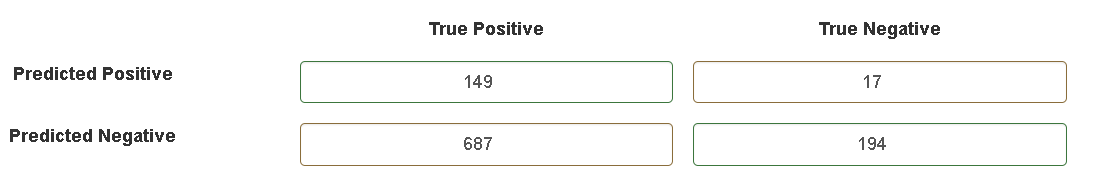
\includegraphics[width=1\columnwidth]{images/ConfusionMatrixEyes.PNG}
 \centering
 \setlength{\abovecaptionskip}{1pt}
 \caption{Confusion Matrix Eyes}
 \label{fig:ConfEyes}
\end{figure}

\begin{figure}[H]
 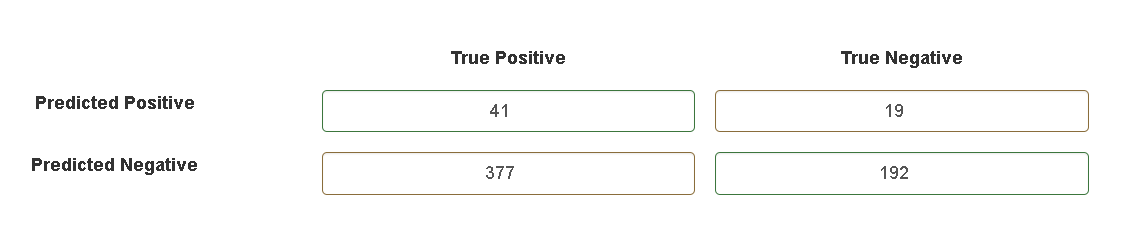
\includegraphics[width=1\columnwidth]{images/ConfusionMatrixSmiles.PNG}
 \centering
 \setlength{\abovecaptionskip}{1pt}
 \caption{Confusion Matrix Smiles}
 \label{fig:ConfSmiles}
\end{figure}



\section*{Conclusion}
We wrote a program for face detection on base of the Viola-Jones-Detection strategy. For this we used Python and the openCV library. First we had the Problem of detecting eyes and smiles everywhere in the pictures. Then after taking the step of detecting the faces first and then looking for eyes and smiles in the faces we got way better results. Lastly after optimizing the values of the parameters of the functions we got a even better result. We had to play around and there was a trade off between finding the actual eyes and smiles and finding fake ones. The program has problems finding faces when they are tilted, small or there is something blocking a part of it. With some changes in the code to cancel out some problems the potential of the detection is high. Improvements of this could be the detection of eyes in just the upper part of the face and smiles just in the lower part of the face, the detection of eyes with similar size and the detection of two eyes per face. Also for detecting smiles we can search in the horizontal middle of the face. One of the most important improvements could be the change of the image size to a optimum to find as many real faces as possible. To conclude we can say there would be some ways to improve our program to find more details which where not detected before, although the program as it is gives us some good results already.

\bibliographystyle{plain}
\bibliography{sources}{}

%\bibliographystyle{ieeetr}



\end{document}
